\documentclass[12pt,a4paper]{article}
\usepackage[UTF8]{ctex} % 支持中文
\usepackage{geometry}
\usepackage{graphicx}
\usepackage{amsmath}
\usepackage{float}
\usepackage{subfigure}
\usepackage{booktabs} % 表格美化
\usepackage{cite}
\usepackage{ulem}
\usepackage{array}
\usepackage{multirow}
\usepackage{hanging}
\def\kong{\hspace*{2em}}

\newcolumntype{M}[1]{>{\centering\arraybackslash}m{#1}}
\newcommand{\down}[2]
{
	$\Delta_{\text{#1}}\approx{#2}$
}

% 设置页面边距
\geometry{left=2.5cm,right=2.5cm,top=2.5cm,bottom=2.5cm}

\title{\Huge{\textbf{\uuline{实\ 验\ 报\ 告}}}}
\author{\uline{少年班}\ 学院 \quad 姓名:\ \uline{顾泓宇} \quad 学号:\ \uline{PB23000078} \quad 实验日期:\ \uline{2024-5-27}}
\date{}

\begin{document}
	\maketitle
	
	\section{实验题目}
	用分光计测三棱镜折射率
	
	\section{实验目的}
	1.了解分光计的结构及工作原理，掌握分光计的调整方法和调节技巧。\\
	\hspace*{2em}2.用最小偏向角法测量玻璃三棱镜的折射率。\\
	\hspace*{2em}3.利用分光计探究三棱镜材料的色散。\\
	\hspace*{2em}4.探究分光计的应用技术和方法。
		
	\section{实验原理}
	\subsection{分光计的结构}
	分光计主要由底座、平行光管、望远镜、载物台和读数圆盘五部分组成，结构如图1所示。\\
	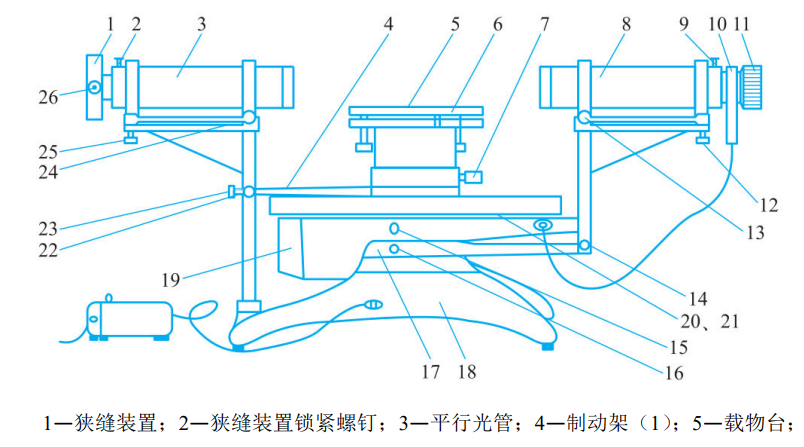
\includegraphics{figs/1.png}\\
	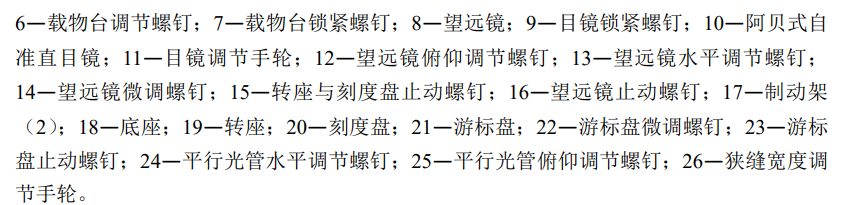
\includegraphics{figs/2.png}
	
	\subsection{分光计的调整原理和方法}
	调整分光计，最后要达到下列要求：\\
	\hspace*{2em}1.望远镜对平行光聚焦.\\
	\hspace*{2em}2.望远镜光轴与仪器主轴垂直.\\
	\hspace*{2em}3.平行光管出射平行光.\\
	\hspace*{2em}4.平行光管光轴与仪器主轴垂直，与望远镜光轴共轴\\
	分光计调整的关键是调好望远镜，其他的调整可以以望远镜为基准。具体的调节方法如下图2、3、4、5.\\
	\begin{minipage}{1\linewidth}
		\centering
		\textbf{图\ 2}\quad 载物台倾角的调整原理与方法 \\[4pt]
		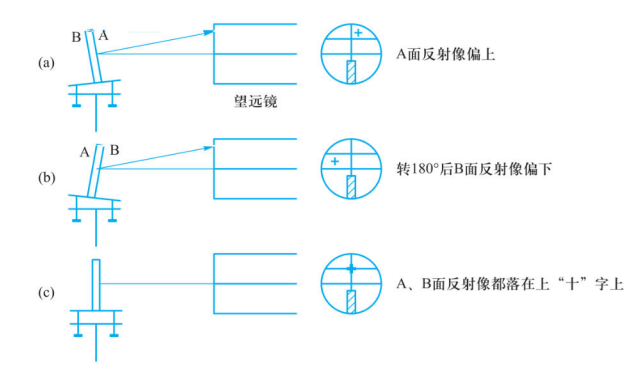
\includegraphics[width=0.8\linewidth]{figs/3.png}
		\label{tp2.png}
	\end{minipage}\\[12pt]
	\begin{minipage}{1\linewidth}
		\centering
		\textbf{图\ 3}\quad 望远镜光轴的调整原理与方法 \\[4pt]
		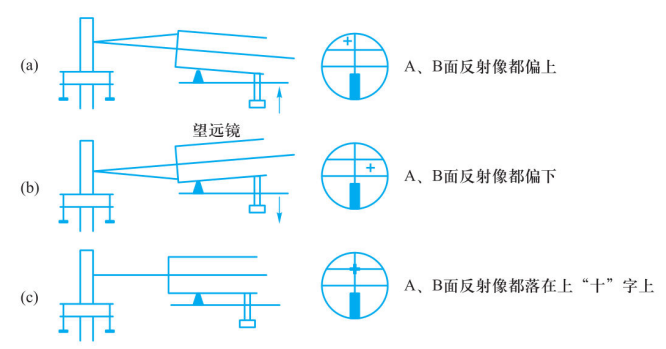
\includegraphics[width=0.8\linewidth]{figs/4.png}
		\label{tp3.png}
	\end{minipage}\\[12pt]
	\begin{minipage}{1\linewidth}
		\centering
		\textbf{图\ 4}\quad 各半调节法调整望远镜光轴与仪器主轴垂直 \\[4pt]
		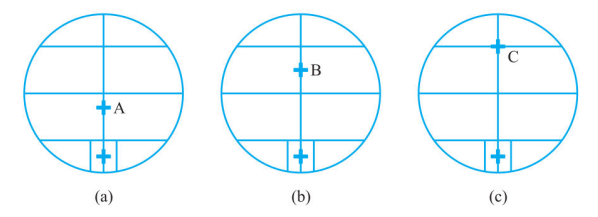
\includegraphics[width=0.8\linewidth]{figs/7.png}
		\label{tp4.png}
	\end{minipage}\\[12pt]
	\begin{minipage}{1\linewidth}
	\centering
	\textbf{图\ 5}\quad 调节平行光管与仪器主轴垂直 \\[4pt]
	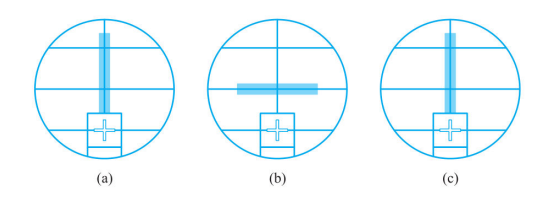
\includegraphics[width=0.8\linewidth]{figs/6.png}
	\label{tp5.png}
	\end{minipage}\\[12pt]
	
	\subsection{用最小偏向角法测三棱镜材料的折射率}
	一束单色光以$i_{1}$角入射到AB面上，经棱镜两次折射后，从AC面射出，出射角为$i_{2}^{\prime}$,如图6.入射光与出射光之间的夹角$\delta$称为偏向角。当棱镜顶角A一定时，偏向角的大小随入射角$i_{1}$的变化而变化。可以证明当$i_{1}=i_{2}^{\prime}$时$\delta$最小。这时的偏向角称为最小偏向角，记为$\delta_{min}$.
	\hspace*{2em}由图6可以看出，这时
	\begin{center}
		$ i_{1}^{\prime}=\frac{A}{2} $
	\end{center}
 	\begin{equation}\label{equ-1}
 		\frac{\delta_{min}}{2}=i_{1}-i_{1}^{\prime}=i_{1}-\frac{A}{2}
 	\end{equation}
 	\begin{center}
 		$ i_{1}=\frac{A+\delta_{min}}{2} $
 	\end{center} 	
	设棱镜材料折射率为n，则
 	\begin{center}
		$ sini_{1}=nsini_{1}^{\prime}=nsin\frac{A}{2} $
	\end{center} 		
	 \begin{equation}\label{equ-2}
		n=\frac{sini_{1}}{sin\frac{A}{2}}=\frac{sin\frac{\delta_{min}+A}{2}}{sin\frac{A}{2}}
	\end{equation}
	由此可知，要求得棱镜材料折射率n，必须测出其顶角A和最小偏向角$\delta_{min}$\\
	\begin{minipage}{1\linewidth}
		\centering
		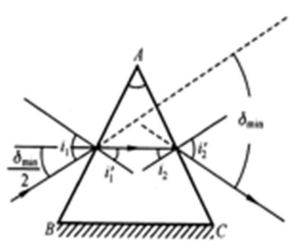
\includegraphics[width=0.8\linewidth]{figs/8.png}\\
		\textbf{图\ 6}\quad 最小偏向角原理图 \\[4pt]
		\label{tp6.png}
	\end{minipage}\\[12pt]

	\subsection{三棱镜的色散及柯西色散公式}
	\subsubsection{三棱镜的色散}
	1672 年牛顿首先利用三棱镜将太阳光分解为彩色光带。让一束白光以一定
	角度从三棱镜侧面入射，由于不同颜色（频率）的光具有不同的折射率，其出
	射光束中不同颜色的光偏向角不同，从而使得不同颜色的光被分离开来，这种
	现象被称为色散。一般而言，光的频率越高，介质对这种光的折射率就越大。
	在可见光中，紫光的频率最高，红光频率最低。当白光通过三棱镜时，棱镜对
	紫光的折射率最大，紫光的偏折程度最大，红光偏折程度最小，见图7。被色
	散开的单色光按波长（或频率）大小而依次排列的图案称为光谱.
	\begin{minipage}{1\linewidth}
		\centering
		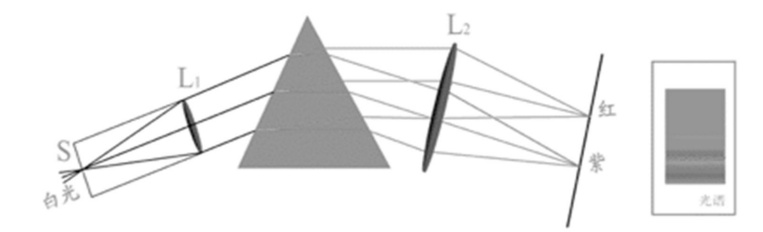
\includegraphics[width=0.8\linewidth]{figs/9.png}\\
		\textbf{图\ 7}\quad 三棱镜的色散 \\[4pt]
		\label{tp7.png}
	\end{minipage}\\[12pt]
	\subsubsection{柯西色散公式}
	1836 年柯西发现材料的折射率和波长的关系，可以用一个经验公式表示：
	\begin{equation}\label{equ-3}
		n(\lambda)=a+\frac{b}{\lambda^2}+\frac{c}{\lambda^4}
	\end{equation}
	其中 a、b、c 是和材料有关的常数。
	
	\subsection{实验装置}
	分光计，汞灯，挡光板，双平面反射镜，三棱镜，放大镜等。
	
	\section{实验内容}
	\subsection{调整分光计}
	要求与调整方法见原理部分
	
	\subsection{使三棱镜光学侧面垂直望远镜光轴}
  	(1)调节载物台调节螺钉 c 使其高度与 a、b 一致，保证载物台大致水平。
	将三棱镜放到载物台上，使棱镜的三个顶角分别对准载物台面下三个底角螺
	钉，见图 8a。\\
	\hspace*{2em}(2)打开目镜照明光源，用挡光板遮住狭缝。转动游标盘，在望远镜中观察
	三棱镜侧面 AB 和 AC 反射回来的绿十字像。如果 AB 面反射的绿十字像与分划
	板上十字线不重合，只调 C 角处的螺钉使之重合；如果 AC 面反射的绿十字像
	与分划板上十字线不重合，只调 B 角处的螺钉使之重合；如此反复几次，直至
	AB 和 AC 面反射的绿十字像都与上十字线重合（切勿调节望远镜俯仰螺钉）。
	此时该三棱镜的主截面垂直仪器主轴，可认为载物台平面垂直仪器主轴。
	注意：每个螺钉的调节要轻微；三棱镜侧面反射的绿十字像亮度较低，观
	察时需要仔细，在较暗的环境中更容易观察清楚。
	\begin{minipage}{1\linewidth}
		\centering
		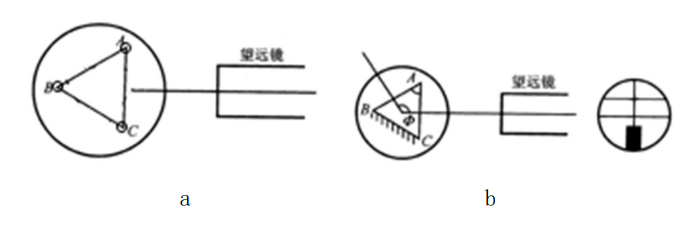
\includegraphics[width=0.8\linewidth]{figs/10.png}\\
		\textbf{图\ 8}\quad 用三棱镜调载物台平面与仪器主轴垂直示意图 \\[4pt]
		\label{tp8.png}
	\end{minipage}\\[12pt]
	
	\subsection{基础内容：测量三棱镜顶角A}
	测量的过程中三棱镜位置要保持不动。对两游标作一适当标记，分别称游
	标 1 和游标 2，切记勿颠倒。旋紧刻度盘下螺钉（15、16），望远镜和刻度盘固
	定不动。转动游标盘，使棱镜 AC 面正对望远镜，见图8b。记下游标 1 的读数$\theta_1$和游标 2 的读数$\theta_2$
	再转动游标盘，使 AB 面正对望远镜，记下游标 1 的读数$\theta_1^{\prime}$和游标 2 的读数$\theta_2^{\prime}$.
	两次读数之差即是载物台转过的角度$\Phi=\frac{1}{2}[\left | \theta_1-\theta_1^{\prime} \right |+\left | \theta_2-\theta_2^{\prime} \right |]$,而$\Phi$是A的补角.\\
	其中P=0.95，n=3时，t=3.18,正态分布$K_{p}=1.960$,均匀分布$K_{p}=1.645$\\
	数据如表一：
	\begin{center}
		\textbf{表\ 一}\quad 测量三棱镜顶角数据  \\[4pt]
		\begin{tabular}{|l|l|l|l|l|l|} \hline
			      & $\theta_{1}$       & $\theta_{2}$       & $\theta_{1}^{\prime}$      & $\theta_2^{\prime}$      & A            						  \\\hline
			第1次 & $182^{\circ}10^{\prime}$ & $2^{\circ}15^{\prime}$ & $62^{\circ}15^{\prime}$ & $242^{\circ}15^{\prime}$  & $60^{\circ}2.5^{\prime}$     \\\hline
			第2次 & $182^{\circ}12^{\prime}$  & $2^{\circ}15^{\prime}$ & $62^{\circ}13^{\prime}$ & $242^{\circ}14^{\prime}$ & $60^{\circ}$ 				\\\hline
			第3次 & $182^{\circ}12^{\prime}$   & $2^{\circ}16^{\prime}$ & $62^{\circ}15^{\prime}$ & $242^{\circ}14^{\prime}$ & $60^{\circ}0.5^{\prime}$ 	\\\hline
		\end{tabular}
	\end{center}
	 $\overline{A}=\frac{1}{3}(60^{\circ}2^{\prime}30^{\prime \prime}+60^{\circ}+60^{\circ}0^{\prime}30^{\prime \prime})=60^{\circ}1^{\prime}30^{\prime \prime}$\\
	 $\sigma_{A}=\sqrt \frac{(A_1-\bar A)^2+(A_2-\bar A)^2++(A_3-\bar A)^2}{3-1}=\frac{\sqrt{34}}{4}^{\prime}$\\
	 则顶角A的A类不确定度为：\\
	 $u_{AA}=\frac{\sigma_{A}}{\sqrt{3}}=0.841^{\prime}$\\
	 $\Delta B=60^{\prime}$\\
	 则伸展不确定度为(P=0.95)：
	 $U_{A}=\sqrt {(3.18\times \frac{\sqrt{34}}{4})^2+(1.645\times \frac{60^{\prime \prime}}{\sqrt 3})^2}=2^{\prime}46^{\prime \prime} $\\
	 $A=60^{\circ}1^{\prime}30^{\prime \prime} \pm 2^{\prime}46^{\prime \prime}$
	 
	 \subsection{提高内容：测量546.1nm谱线对应最小偏向角计算折射率}
	 (1) 平行光管狭缝对准前方汞灯光源。\\
	 \kong (2) 旋松望远镜止动螺钉和游标盘止动螺钉，把载物台及望远镜转至所示位置，再左右微微转动望远镜，找
	 出棱镜出射的各种颜色的汞灯光谱线（各种波长的狭缝像）。 (3) 轻轻转动载物台，改变入射角$i_{1}$,在望远镜
	 中将看到谱线跟着动。改变$i_{1}$,应使谱线往$\delta$减小的方向移动(向顶角A方向移动)。。望远镜要跟踪光谱线转动，
	 直到棱镜继续转动，而谱线开始要反向移动（即偏向角反而变大）为止。这个反向移动的转折位置，就是光线以最小偏向角射出的方向。固定载物台，再使望远镜微动，使其分划板上的中心竖线对准其中的那条绿谱线（546.1nm）(见图9)。\\
	 \kong (3)记下此时两游标处的读数$\theta_{1}$和$\theta_{2}$。取下三棱镜（载物台保持不动），转动望远镜对准平行发光管，以确定入射光的方向，再记下两游标处的读数$\theta_{1}^{\prime}$和$\theta_{2}^{\prime}$。此时绿色谱线的最小偏向角为$\delta_{min}=[|\theta_1-\theta^{\prime}_1|+|\theta_2-\theta^{\prime}_2|]/2$。\\
	 \begin{minipage}{1\linewidth}
	 	\centering
	 	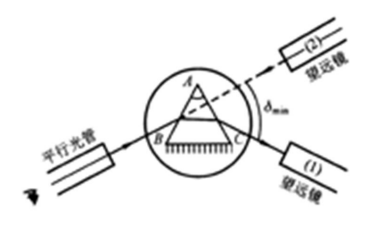
\includegraphics[width=0.8\linewidth]{figs/11.png}\\
	 	\textbf{图\ 9}\quad 测最小偏向角方法 \\[4pt]
	 	\label{tp9.png}
	 \end{minipage}\\[12pt]
	 数据如表二：
	 \begin{center}
	 	\textbf{表\ 二}\quad 测量546.1nm谱线对应最小偏向数据角  \\[4pt]
	 	\begin{tabular}{|l|l|l|l|l|l|} \hline
	 			  & $\theta_{1}$      		  & $\theta_{2}$       & $\theta_{1}^{\prime}$        & $\theta_2^{\prime}$      & $\delta_{min}$            	\\\hline
	 		第1次 & $60^{\circ}5^{\prime}$ 	& $240^{\circ}5^{\prime}$ & $21^{\circ}11^{\prime}$ & $201^{\circ}11^{\prime}$  & $38^{\circ}54^{\prime}$     \\\hline
	 		第2次 & $60^{\circ}4^{\prime}$ 	& $240^{\circ}5^{\prime}$ & $21^{\circ}10^{\prime}$ & $201^{\circ}9^{\prime}$   & $38^{\circ}55^{\prime}$ 	  \\\hline
	 		第3次 & $60^{\circ}3^{\prime}$  	& $240^{\circ}4^{\prime}$ & $21^{\circ}9^{\prime}$  & $201^{\circ}8^{\prime}$   & $38^{\circ}56^{\prime}$ 	  \\\hline
	 	\end{tabular}
	 \end{center}
	 $\overline{\delta_{min}}=\frac{1}{3}(38^{\circ}54^{\prime}+38^{\circ}55^{\prime}+38^{\circ}56^{\prime})=38^{\circ}55^{\prime}$\\
	 $\sigma_{\delta_{min}}=\sqrt \frac{(\delta_{1,min}-\bar \delta_{min})^2+(\delta_{2,min}-\bar \delta_{min})^2++(\delta_{3,min}-\bar \delta_{min})^2}{3-1}=1^{\prime}$\\
	 则最小偏向角$\theta_{min}$的A类不确定度为：\\
	 $u_{A\theta}=\frac{\sigma_{\theta_{min}}}{\sqrt{3}}=0.577^{\prime}$\\
	 $\Delta B=60^{\prime}$\\
	 则伸展不确定度为(P=0.95)：
	 $U_{\delta_{min}}=\sqrt {(3.18\times 1)^2+(1.645\times \frac{60^{\prime \prime}}{\sqrt 3})^2}=3^{\prime}19^{\prime \prime} $\\
	 则$\delta_{min}=38^{\circ}55^{\prime} \pm 3^{\prime}19^{\prime \prime}$\\
	 由公式(2)，得$ n=\frac{\sin\frac{\delta _{min}+A}{2}}{\sin\frac {A}{2}}=1.521$\\
	 对上式做全微分，得$\frac{\Delta n}{n}=\frac{1}{2}(\cot\frac{\delta _{min}+A}{2}-\cot\frac A 2)\Delta A+\frac{1}{2} \cot\frac{\delta _{min}+A}{2}\Delta \delta_{min}$\\
	 计算得$U_{n}=n\sqrt{\frac{ 1 }{4}(\cot\frac{\delta _{min}+A}{2}-\cot\frac{ A }{2})^2\Delta A^2+\frac {1} {4} \cot^2\frac{\delta _{min}+A}{2}\Delta \delta_{min}^2}=0.0202$\\
	 即$n=1.521 \pm 0.0202$。
	 
	 \subsection{进阶内容：计算三棱镜材料对应柯西色散系数}
	 除已经测得的汞灯绿色谱线外，再测量汞灯其他谱线（435.8 nm 紫
	 色谱线，577.0 和 579.0 nm黄色双线）的最小偏向角，并求出相应的折射率。利用所测得不同波长谱线的折射率和公式(3)，求出三棱镜材料的柯西色散系数。
	 数据如表三：
	 \begin{center}
	 	\textbf{表\ 二}\quad 测量546.1nm谱线对应最小偏向数据角  \\[4pt]
	 	\begin{tabular}{|l|l|l|l|l|l|} \hline
	 			  & $\theta_{1}$      		  & $\theta_{2}$       & $\theta_{1}^{\prime}$        & $\theta_2^{\prime}$      & $\delta_{min}$            	\\\hline
	 		内黄线 & $59.5^{\circ}22^{\prime}$	& $239^{\circ}59^{\prime}$ & $21^{\circ}10^{\prime}$ & $201^{\circ}9^{\prime}$  & $38.25^{\circ}21^{\prime}$     \\\hline
	 		外黄线 & $59.5^{\circ}23^{\prime}$ 	& $240^{\circ}$ & $21^{\circ}10^{\prime}$ & $201^{\circ}9^{\prime}$   & $38.25^{\circ}32^{\prime}$ 	  \\\hline
	 		紫线   & $60.15^{\circ}15^{\prime}$  	& $240.5^{\circ}20^{\prime}$ & $21^{\circ}9^{\prime}$  & $201^{\circ}8^{\prime}$   & $39.5^{\circ}8^{\prime}$ 	  \\\hline
	 	\end{tabular}
	 \end{center}
	 由公式(2)计算得$n_{\text{内黄}}=1.517$，$n_{\text{外黄}}=1.518$，$n_{\text{紫}}=1.527$\\
	 代入柯西色散公式，解线性方程组得：a=1.421; b=$4.827 \times 10^{-14}$; c=$-5.356 \times 10^{-27}$
	
	\section{思考题}
	1.平面反射镜正反两面反射的十字像分别在叉丝上方 3a 处和下方 a 处，试作图分析，提出能迅速使望远镜光轴与仪器主轴垂直的调节方法。\\
	\kong 答：见下图\\
	\begin{minipage}{1\linewidth}
		\centering
		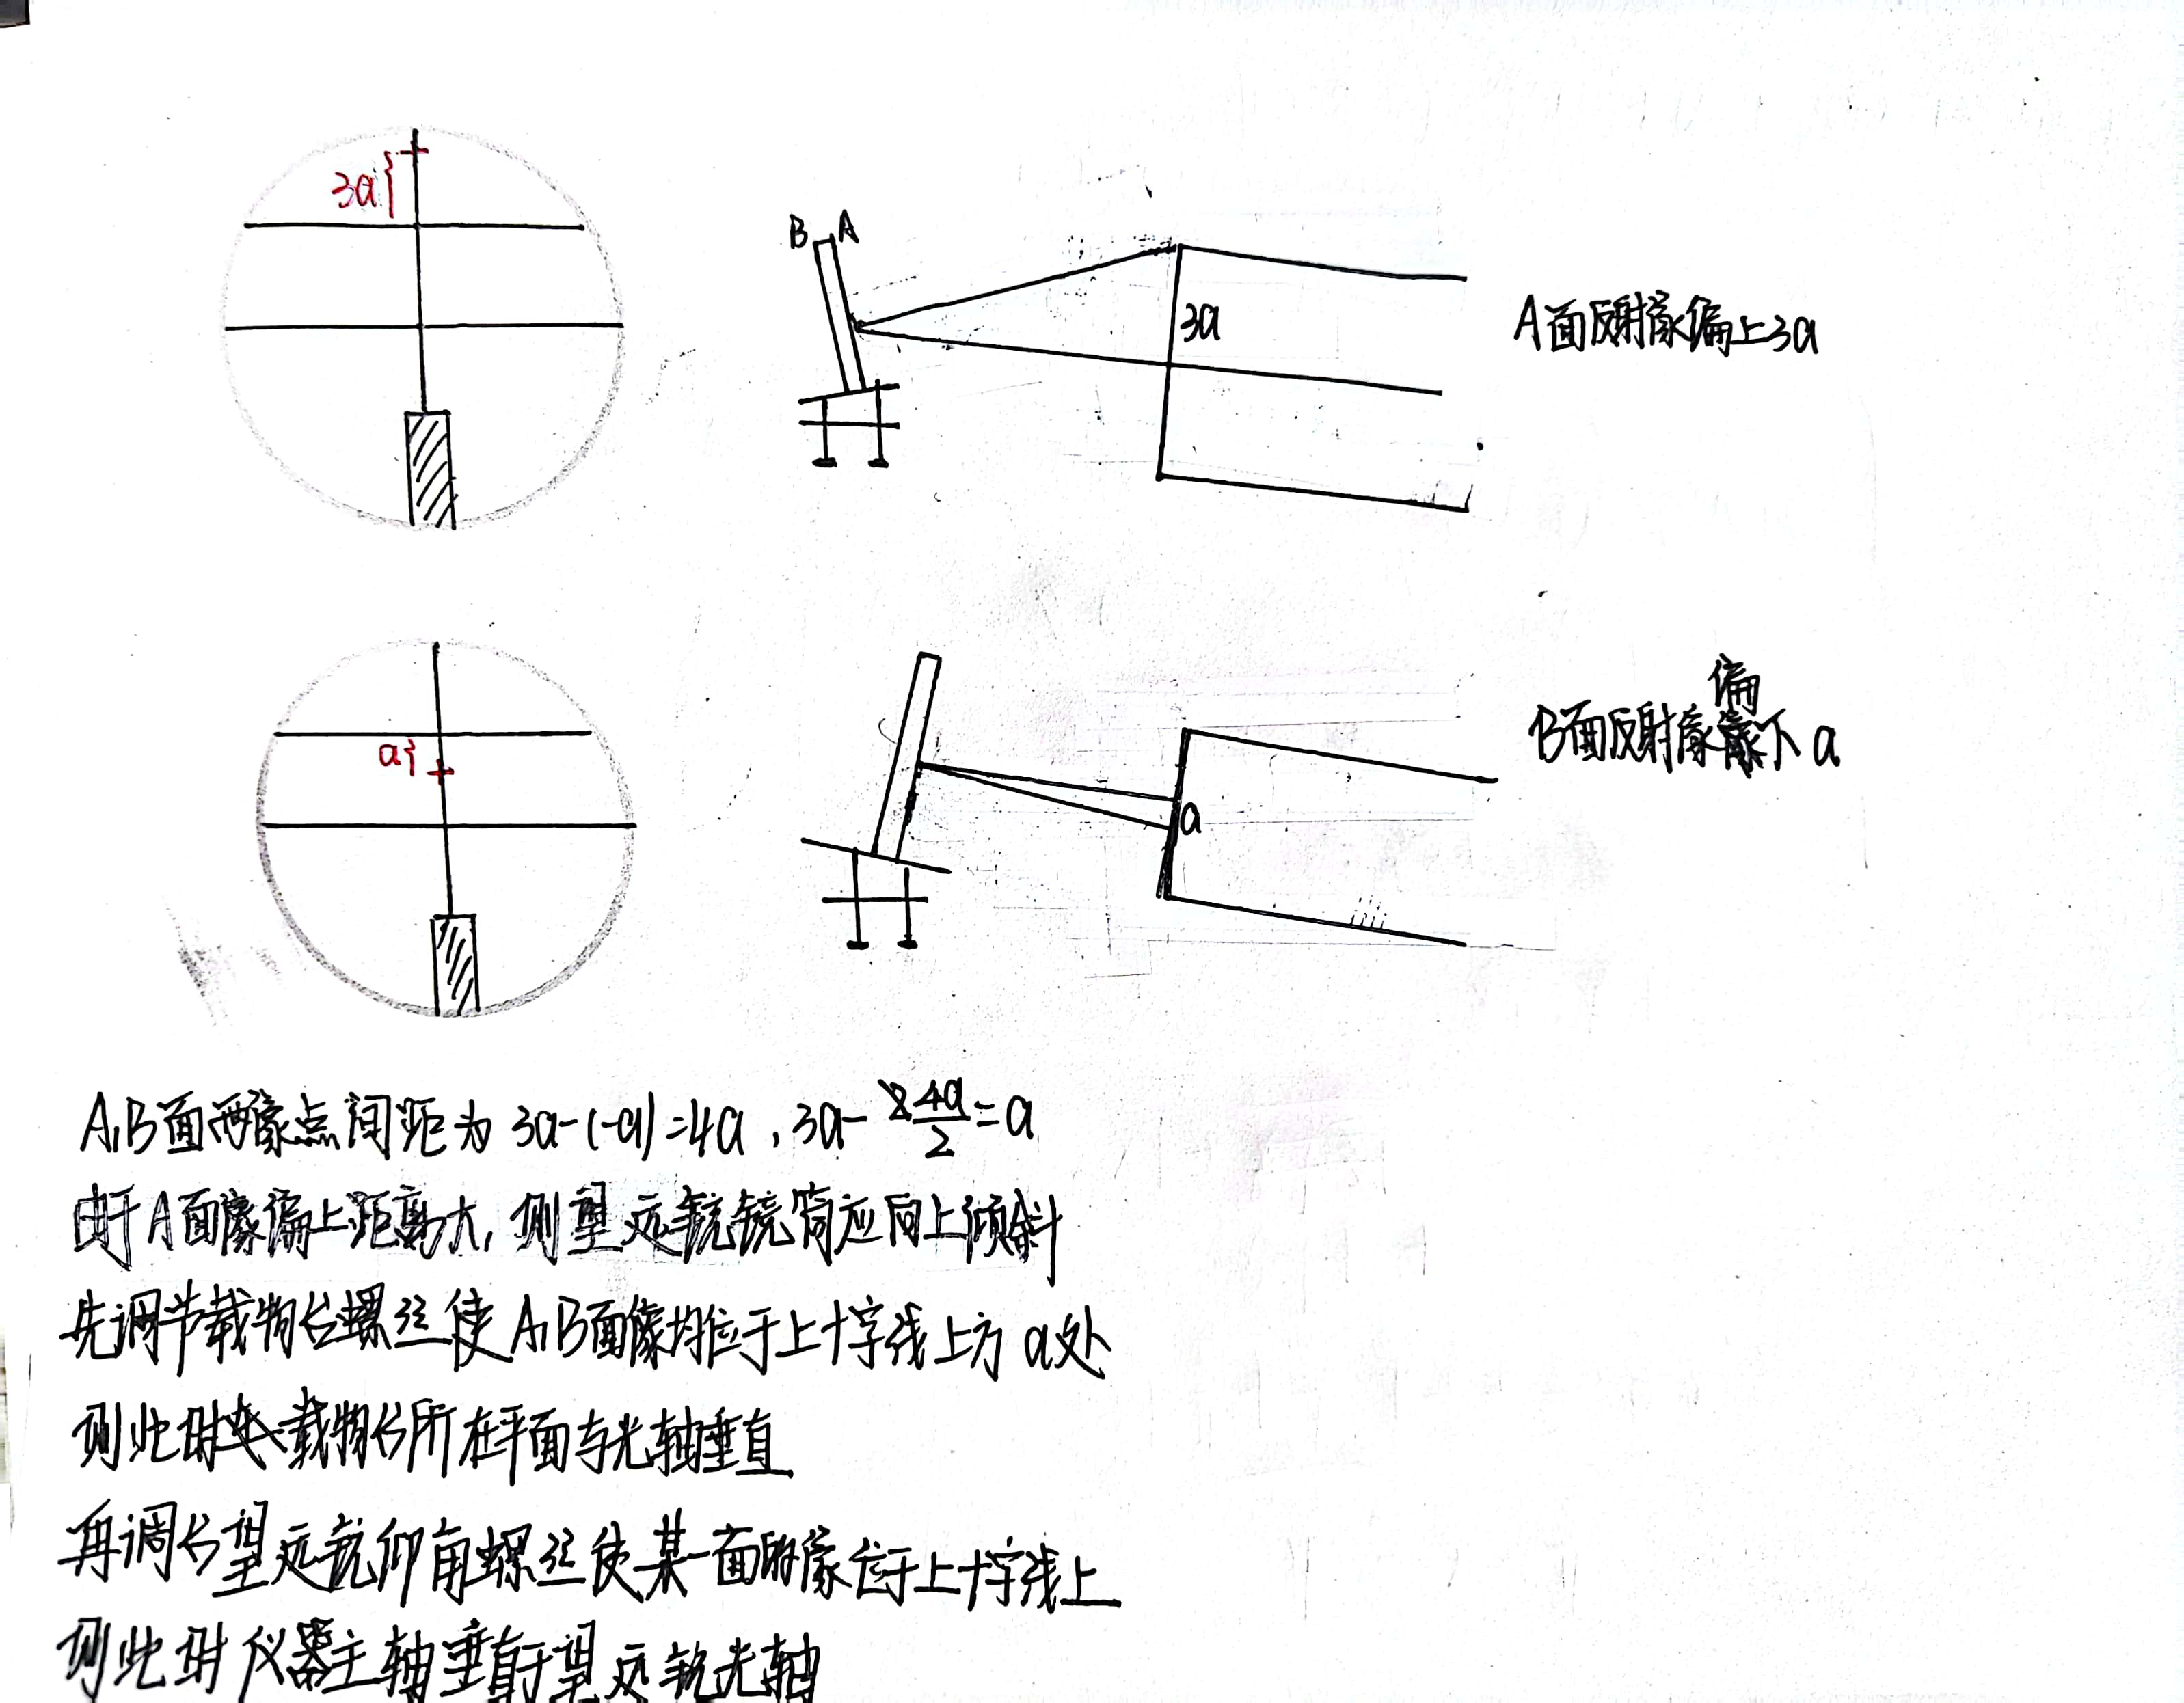
\includegraphics[width=0.8\linewidth]{figs/14.jpg}
	\end{minipage}\\[12pt]
	
	2.在寻找最小偏向角的过程中，可以发现在处于最小偏向角附近时偏向角对入射角的大小变化不敏感，这会降低最小偏向角的测量精度吗？为什么?\\
	\kong 答：会降低测量精度，因为由于偏向角对入射角变化不敏感，会出现手动调节时入射角时入射角有较大变化但偏向角变化不明显，从而难以准确确认最小偏向角所对应的入射角位置，再根据$\delta_{min}=[|\theta_1-\theta^{\prime}_1|+|\theta_2-\theta^{\prime}_2|]/2$，入射角测量的误差会影响最小偏向角的测量精度。
	
	\begin{thebibliography}{2}
	\bibitem{ref1} 分光计的调整与使用(1303实验室). 实验讲义.2024 
	\bibitem{ref2} 用分光计测量三棱镜的折射率(1303实验室).实验讲义.2024
	\end{thebibliography}
	\section{附录:原始数据记录}
	\begin{minipage}{1\linewidth}
		\centering
		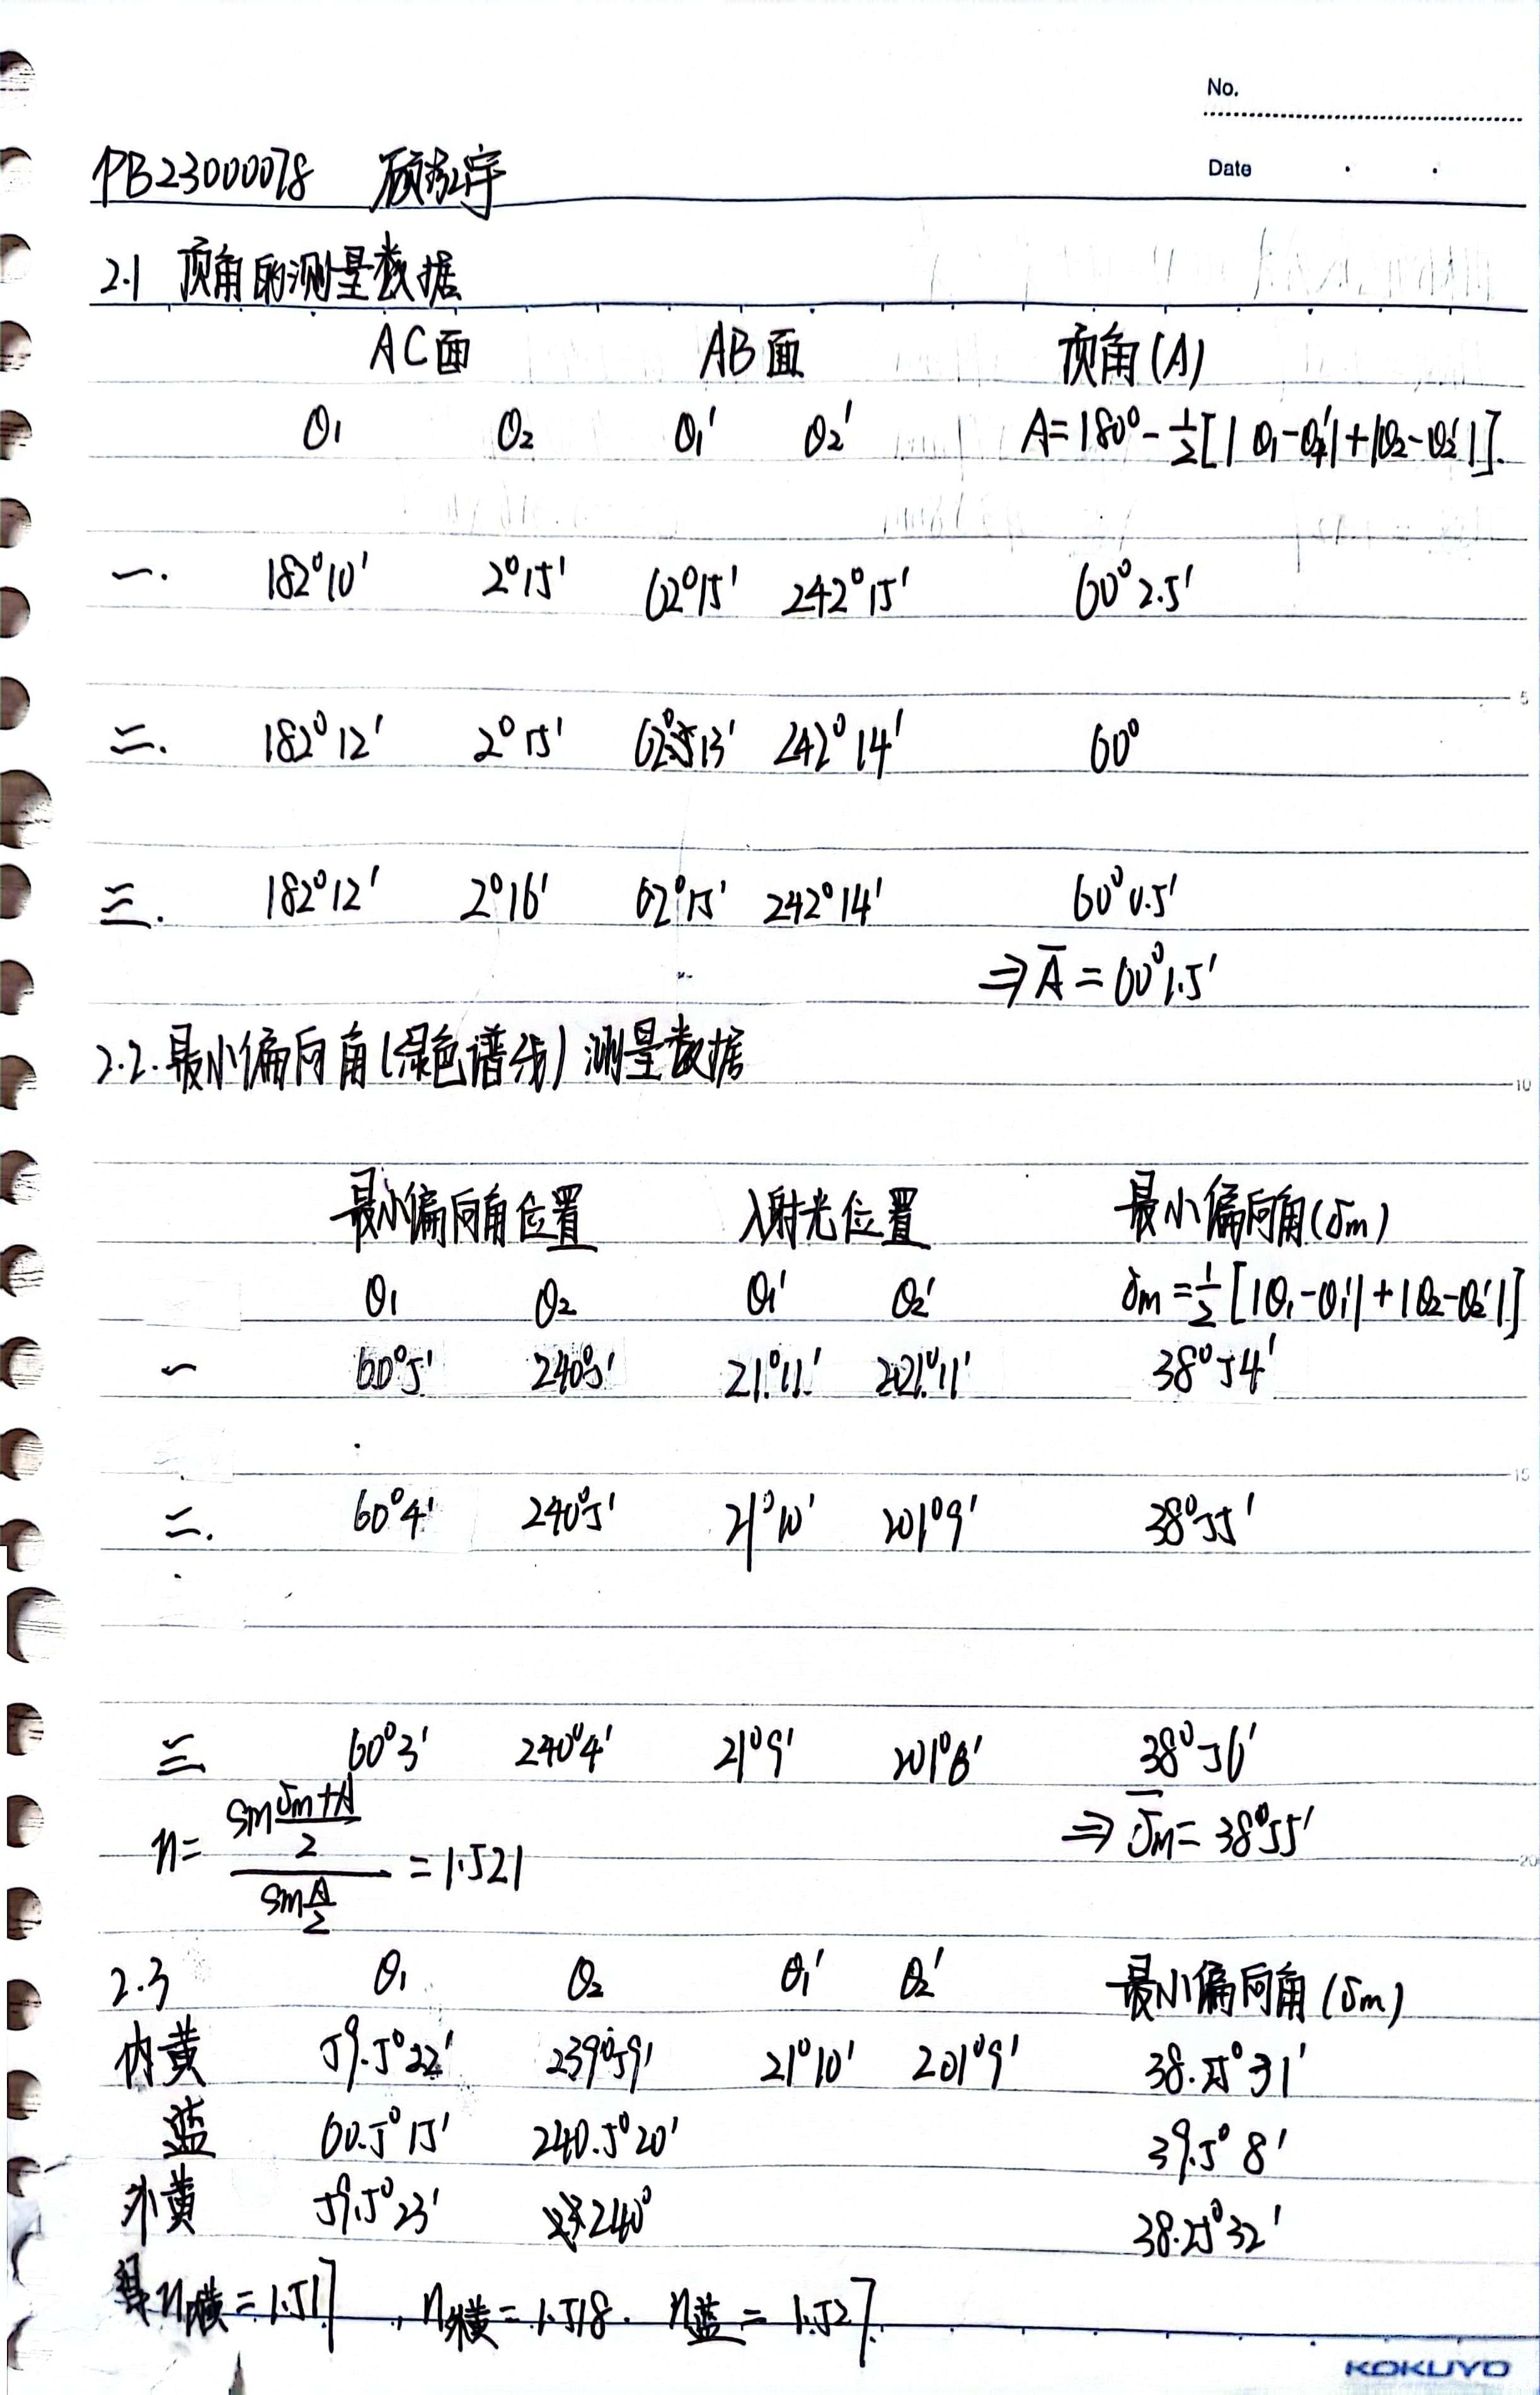
\includegraphics[width=0.6\linewidth]{figs/12.jpg}
	\end{minipage}\\[12pt]
	
	\begin{minipage}{1\linewidth}
	\centering
	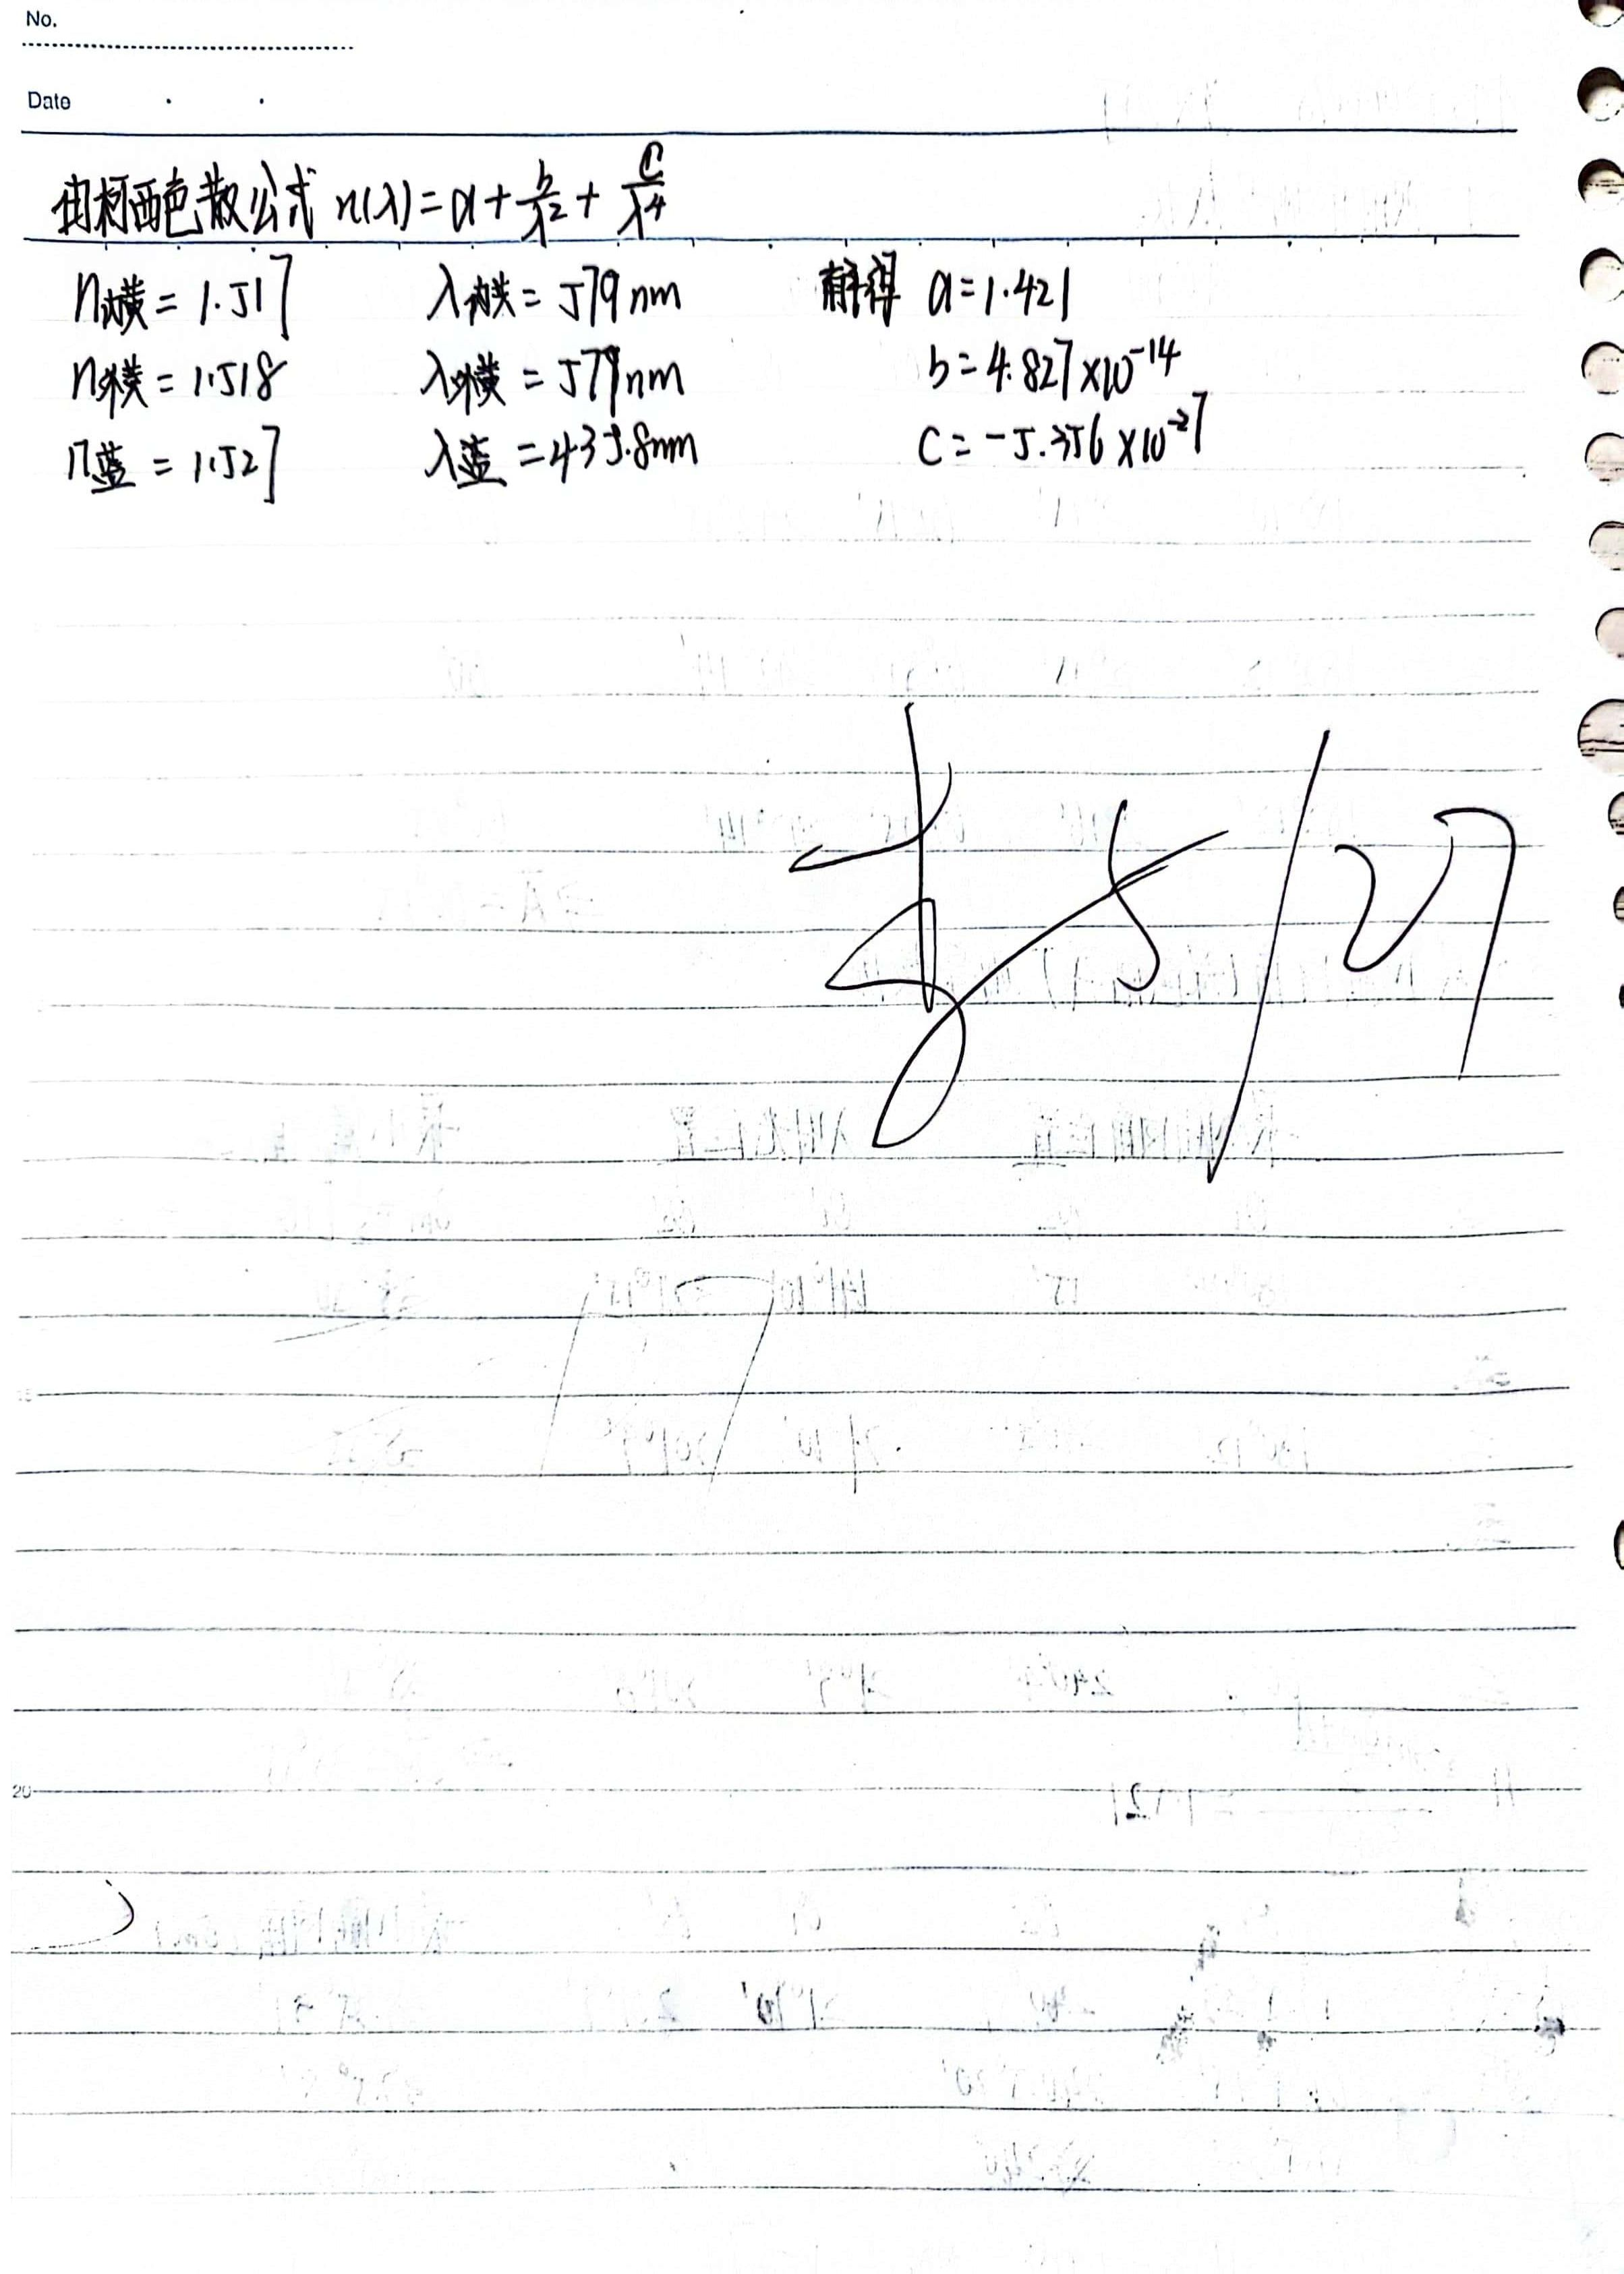
\includegraphics[width=0.6\linewidth]{figs/13.jpg}
	\end{minipage}\\[12pt]
	
\end{document}